\subsubsection{UC2.2 - Inserimento informazioni ristorante amministratore}\label{usecase:2_2}

\begin{figure}[H]
    \centering
    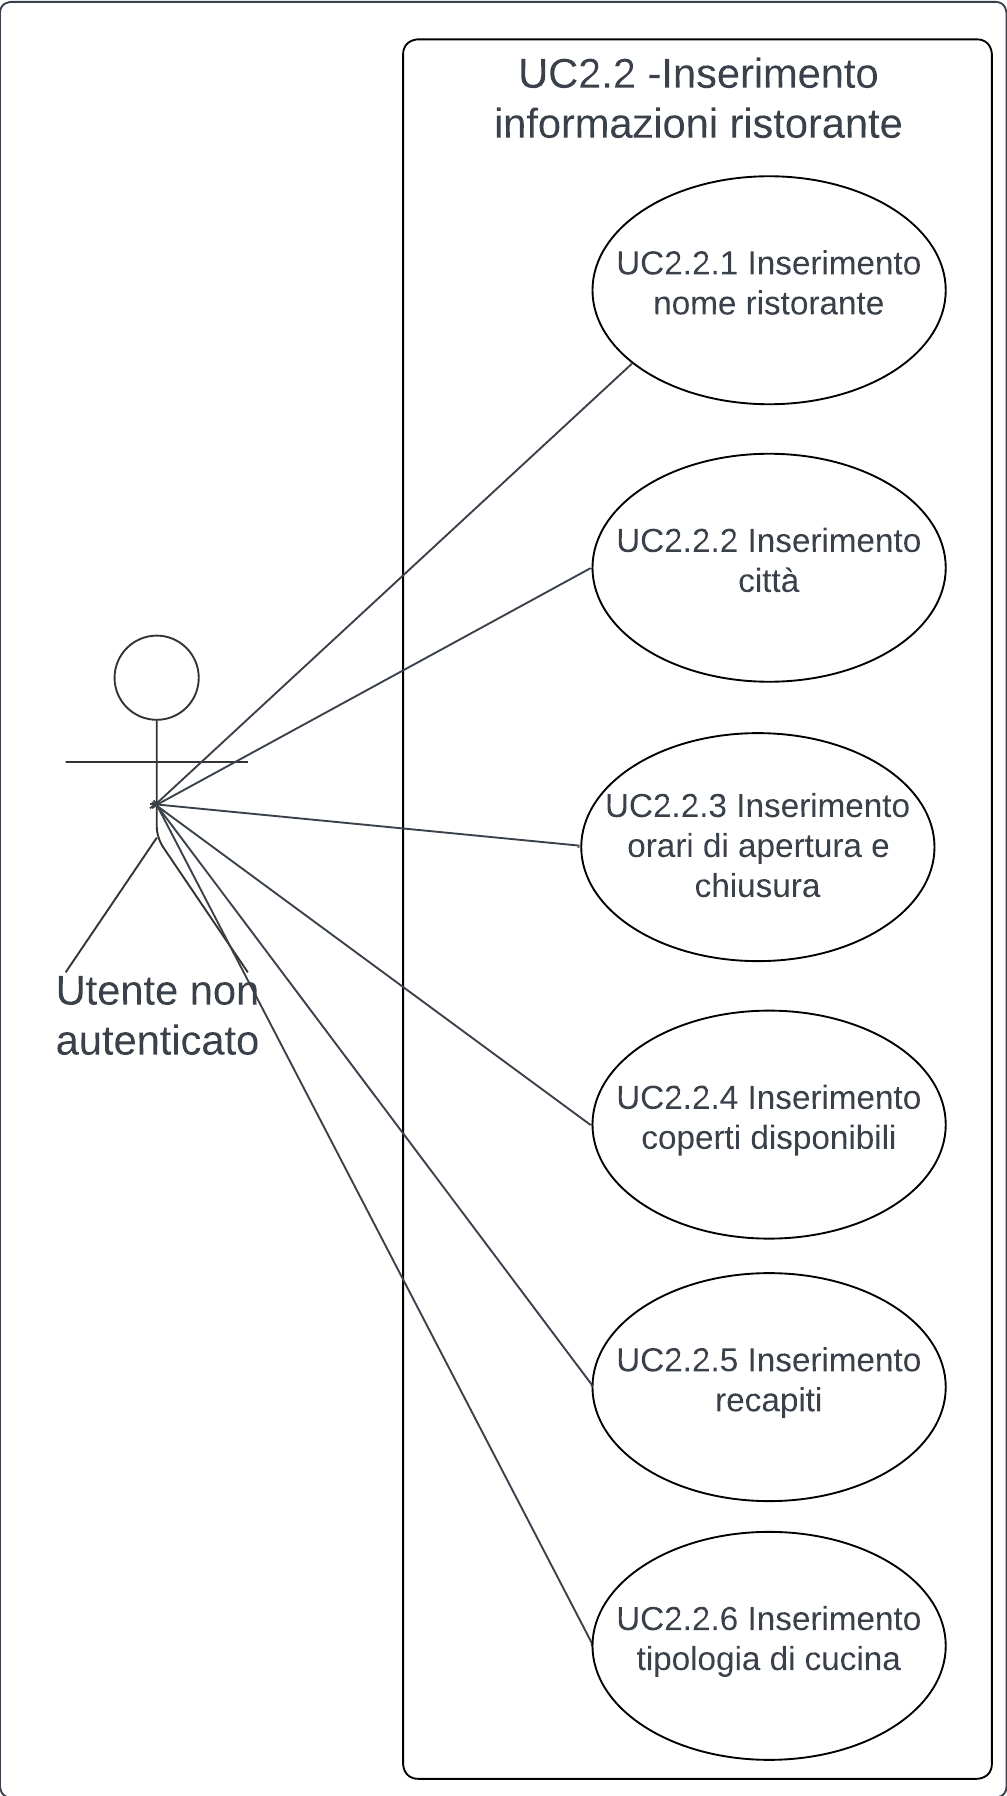
\includegraphics[scale=0.7]{ucd/UCD2.2_finale.png}
\caption{Registrazione come amministratore}
\end{figure}

\textbf{Attori}:
\begin{itemize}
    \item Utente non autenticato.
\end{itemize}
\textbf{Precondizioni}:
\begin{itemize}
    \item L'utente è connesso al $\textit{Sistema}_G$;
    \item L'utente ha ricevuto un link di invito speciale che permette la registrazione come amministratore.
\end{itemize}
\textbf{Postcondizioni}:
\begin{itemize}
    \item L'utente ha inserito le informazioni del ristorante da registrare.
\end{itemize}
\textbf{Scenario principale}:
\begin{enumerate}
    \item L'utente inserisce il nome del ristorante (\nameref{usecase:2_2_1});
    \item L'utente inserisce la città (\nameref{usecase:2_2_2}); 
    \item L'utente inserisce l'orario apertura e chiusura (\nameref{usecase:2_2_3});
    \item L'utente inserisce i coperti disponibili (\nameref{usecase:2_2_4});
    \item L'utente inserisce i recapiti del ristorante (\nameref{usecase:2_2_5});
    \item L'utente inserisce la tipologia di cucina (\nameref{usecase:2_2_6}).
\end{enumerate}
\textbf{Scenari secondari}:
    \begin{enumerate}
        \item L'utente lascia dei campi vuoti;
        \item L'utente inserisce dati non validi.
    \end{enumerate}

\subsubsection{UC2.2.1 - Inserimento nome ristorante}\label{usecase:2_2_1}
\textbf{Attori}:
\begin{itemize}
    \item Utente non autenticato.
\end{itemize}
\textbf{Precondizioni}:
\begin{itemize}
    \item L'utente è connesso al $\textit{Sistema}_G$;
    \item L'utente ha ricevuto un link di invito speciale che permette la registrazione come amministratore.
\end{itemize}
\textbf{Postcondizioni}:
\begin{itemize}
    \item L'utente ha inserito il nome del ristorante
\end{itemize}
\textbf{Scenario principale}:
\begin{enumerate}
    \item L'utente inserisce il nome del ristorante;
\end{enumerate}
\textbf{Scenario secondario}:
\begin{enumerate}
    \item L'utente lascia il nome vuoto;
    \item L'utente usa solo spazi (" ");
    \item L'utente usa caratteri speciali;
\end{enumerate}
\subsubsection{UC2.2.2 - Inserimento città}\label{usecase:2_2_2}
\textbf{Attori}:
\begin{itemize}
    \item Utente non autenticato.
\end{itemize}
\textbf{Precondizioni}:
\begin{itemize}
    \item L'utente è connesso al $\textit{Sistema}_G$;
    \item L'utente ha ricevuto un link di invito speciale che permette la registrazione come amministratore.
\end{itemize}
\textbf{Postcondizioni}:
\begin{itemize}
    \item L'utente ha inserito la città
\end{itemize}
\textbf{Scenario principale}:
\begin{enumerate}
    \item L'utente inserisce il nome della città
\end{enumerate}
\textbf{Scenario secondario}:
\begin{enumerate}
    \item L'utente lascia il campo vuoto;
    \item L'utente usa solo spazi (" ");
    \item L'utente usa caratteri speciali;
\end{enumerate}
\subsubsection{UC2.2.3 - Inserimento orari di apertura e chiusura}\label{usecase:2_2_3}
\textbf{Attori}:
\begin{itemize}
    \item Utente non autenticato.
\end{itemize}
\textbf{Precondizioni}:
\begin{itemize}
    \item L'utente è connesso al $\textit{Sistema}_G$;
    \item L'utente ha ricevuto un link di invito speciale che permette la registrazione come amministratore.
\end{itemize}
\textbf{Postcondizioni}:
\begin{itemize}
    \item L'utente ha gli orari
\end{itemize}
\textbf{Scenario principale}:
\begin{enumerate}
    \item L'utente inserisce l'orario di apertura
    \item L'utente inserisce l'orario di chiusura
\end{enumerate}
\textbf{Scenario secondario}:
\begin{enumerate}
    \item L'utente lascia il campo vuoto;
    \item L'utente inserisce un orario non valido;
\end{enumerate}
\subsubsection{UC2.2.4 - Inserimento coperti disponibili}\label{usecase:2_2_4}
\textbf{Attori}:
\begin{itemize}
    \item Utente non autenticato.
\end{itemize}
\textbf{Precondizioni}:
\begin{itemize}
    \item L'utente è connesso al $\textit{Sistema}_G$;
    \item L'utente ha ricevuto un link di invito speciale che permette la registrazione come amministratore.
\end{itemize}
\textbf{Postcondizioni}:
\begin{itemize}
    \item L'utente ha inserito i coperti
\end{itemize}
\textbf{Scenario principale}:
\begin{enumerate}
    \item L'utente inserisce il numero di coperti
\end{enumerate}
\textbf{Scenario secondario}:
\begin{enumerate}
    \item L'utente lascia il campo vuoto;
    \item L'utente utilizza caratteri diversi dai numeri;
    \item L'utente inserisce un numero non valido (troppo grandi oppure zero)
\end{enumerate}
\subsubsection{UC2.2.5 - Inserimento recapiti}\label{usecase:2_2_5}
\textbf{Attori}:
\begin{itemize}
    \item Utente non autenticato.
\end{itemize}
\textbf{Precondizioni}:
\begin{itemize}
    \item L'utente è connesso al $\textit{Sistema}_G$;
    \item L'utente ha ricevuto un link di invito speciale che permette la registrazione come amministratore.
\end{itemize}
\textbf{Postcondizioni}:
\begin{itemize}
    \item L'utente inserisce i recapiti
\end{itemize}
\textbf{Scenario principale}:
\begin{enumerate}
    \item L'utente inserisce email del ristorante
    \item L'utente inserisce il numero del ristorante
\end{enumerate}
\textbf{Scenario secondario}:
\begin{enumerate}
    \item L'utente lascia i campi vuoti;
    \item L'utente inserisce un numero non valido;
\end{enumerate}
\subsubsection{UC2.2.6 - Inserimento tipologia di cucina}\label{usecase:2_2_6}
\textbf{Attori}:
\begin{itemize}
    \item Utente non autenticato.
\end{itemize}
\textbf{Precondizioni}:
\begin{itemize}
    \item L'utente è connesso al $\textit{Sistema}_G$;
    \item L'utente ha ricevuto un link di invito speciale che permette la registrazione come amministratore.
\end{itemize}
\textbf{Postcondizioni}:
\begin{itemize}
    \item L'utente ha inserito la tipologia di cucina
\end{itemize}
\textbf{Scenario principale}:
\begin{enumerate}
    \item L'utente sceglie la tipologia della cucina del ristorante
\end{enumerate}
\newpage